\chapter{Application layer und Use Cases\label{chap:usecases}}
\section{Application Layer \label{sec:applicationLayer}}
\begin{figure}[htbp]
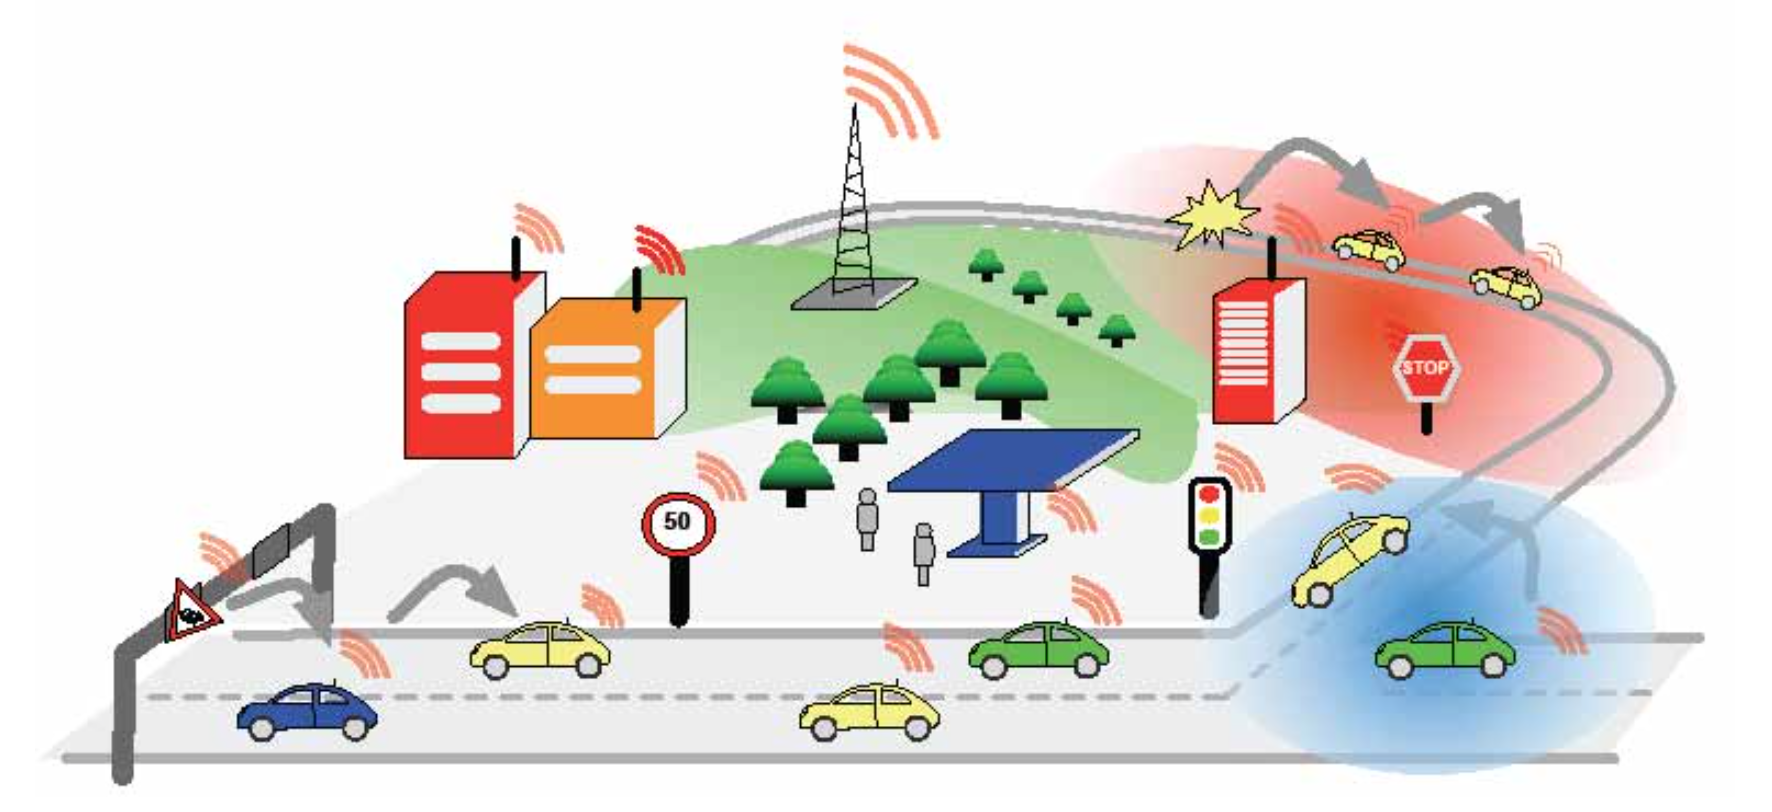
\includegraphics[width=0.95\textwidth]{content/images/06_use_cases/komponenten.png}
\caption{Die Komponenten der \acl{C2C} \cite{etsi102638}}
\label{fig:komponentenderc2x}
\end{figure}
Die \acl{C2C} bietet eine große Vielfalt an verschiedenen Ein\-satz\-mög\-lich\-keit\-en. Das gesamte Projekt ist nicht nur darauf ausgelegt, dass Fahrzeuge untereinander kommunizieren, sondern, wie in der \autoref{fig:komponentenderc2x} zu erkennen, auch andere Verkehrskomponenten. Um das Zusammenspiel der Komponenten besser zu verstehen und zu sehen, wie groß das Potential der \acl{C2C} ist, werden im Folgenden mehrere Szenarien aufgezählt und erklärt. Der Applicationlayer unterscheidet dabei drei Kategorien von Anwendungsfällen. Dazu gehören die Sicherheitsbedingten, die Verkehrseffizienz und die Kategorie Infotainment und Andere.

Der Applicationlayer ist der Layer, der die Applications ausführt. Er hat die Schnittstellen zu dem Management Layer, zu dem Security Layer und dem Facilities Layer. Den Applications bietet er eine Nutzung der Dienste der anderen Layer. 

\section{Use cases}
\subsection{Sicherheitsbedingt}
Sicherheitsbedingte Use Cases sind Anwendungsfälle, bei denen ein möglicher Unfall verhindert werden kann. Im Folgenden werden drei Szenarien erklärt, durch diese das Unfallrisiko minimiert werden kann.

\subsubsection{Cooperative Forward Collision Warning}
Einer der häufigsten Ursachen für Verkehrsunfälle sind plötzliche Bremsmanöver von vorrausfahrenden Fahrzeugen und die Unaufmerksamkeit eines Fahrers. Aus diesen Ursachen resultiert ein erhöhtes Risiko für Auffahrunfälle. Cooperative Forward Collision Warning versucht genau dieses Risiko zu vermindern. Um dies zu erreichen, überwacht jedes Fahrzeug die eigenen Informationen, wie die Geschwindigkeit, Richtung und Position und vergleicht diese mit den Daten der anderen Fahrzeuge. Bei Auffälligkeiten und Abweichungen warnt das System dem Fahrer frühzeitig vor einer möglichen Kollision. Diese Warnung kann durch auditive, visuelle oder haptische Alarme signalisiert werden. Da es durchaus sein kann, dass noch Fahrzeuge, die nicht in dem \ac{ITS} Netz kommunizieren, unterwegs sind, werden die Daten von Objekterkennungssensoren ausgewertet. Dadurch wird das Risiko einer Kollision für die \ac{IVS} weiter reduziert. Die Informationen werden innerhalb von 20 bis 200 Meter mit den anderen \ac{ITS-S} geteilt. Dadurch bleibt den \ac{IVS} genug Zeit um sie auszuwerten und die Fahrer zu warnen.


Nachfolgend wird gezeigt, wie die Use Cases im Standard definiert werden.


\textbf{Application name:} Co-operative collision avoidance or mitigation.

\textbf{Short description:} This use case is based on co-operation between vehicles which detect a risk of forward collision.
Such co\-operation is achieved to avoid accident either through driver assistance of direct action on the cars.

\textbf{Usage:} Avoid longitudinal collision.

\textbf{Communication mode:} V2X co\-operative awareness associated to unicast.

\begin{figure}[htbp]
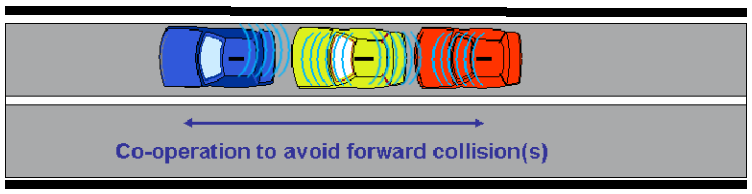
\includegraphics[width=0.95\textwidth]{content/images/06_use_cases/colissionwarning.png}
\caption{Cooperative Forward Collision Warning Use Case \cite{etsi102638}}
\label{fig:cfcw}
\end{figure}

\textbf{Main requirements}
\begin{itemize}
\item Capability for a vehicle to broadcast V2X co-operative awareness messages.
\item Capability for this vehicle to establish unicast Peer to Peer sessions to co-operate with other vehicles closely
\item Maximum latency time: 100 ms.
\item Minimum frequency of V2V co-operation awareness messages: 10 Hz.
\item Authenticity of V2X co-operative awareness messages.
\item Vehicles relative positioning accuracy: < 1 m.
following the same path to reduce the risk of accident.
\end{itemize}

\subsubsection{Pre-Crash Sensing/Warning}
Natürlich können nicht alle Unfälle durch die Cooperative Forward Collision Warning vermieden werden. Es ist davon auszugehen, dass dennoch Auffahrunfälle geschehen werden. Dafür hat man sich das Pre-Crash Sensing/Warning Szenario ausgedacht, bei dem man von einem unvermeidbaren Unfall ausgeht. Dieser soll durch \ac{ITS} erkannt werden. Nach dem Erkennen sollen Vorbereitungen zur Reduzierung der Unfallschäden getroffen werden. Damit dieses System funktioniert, müssen, wie bei dem vorherigen Szenario, dauerhaft Informationen zwischen den \ac{IVS} ausgetauscht werden. Dabei geht man davon aus, dass die Informationen der Fahrzeuge, die sich im Umkreis von 20 bis 100 Meter befinden, überwacht werden müssen. Entdeckt das System einen unvermeidbaren Unfall, muss sichergestellt sein, dass die Fahrzeuge, die kollidieren werden, sicher miteinander kommunizieren können. Dabei werden Daten wie die Fahrzeuggröße, und genaue Position bekannt gegeben. Anhand dieser Informationen können dann Sicherheitsmaßnahmen, wie Airbag, Gurtstraffer oder erweiterbare Stoßstangen gesteuert und effektiv genutzt werden. 

\begin{figure}[htbp]
	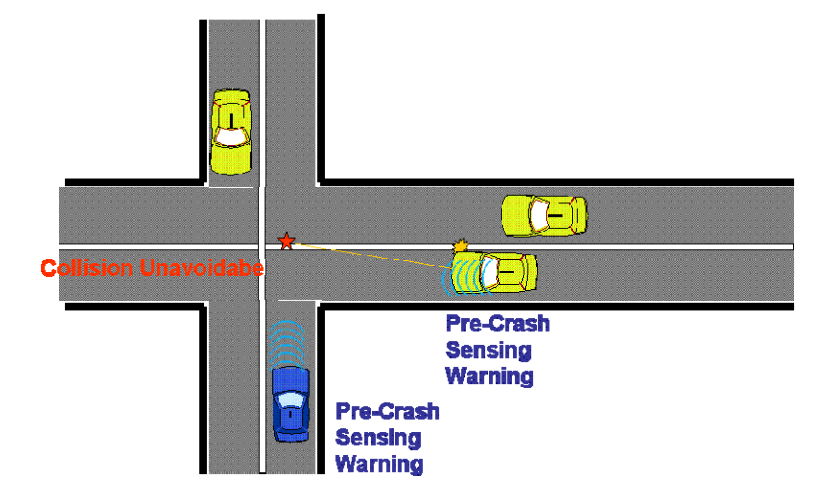
\includegraphics[width=0.95\textwidth]{content/images/06_use_cases/pre_crash_sensing.png}
	\caption{Pre-Crash Sensing/Warning Use Case \cite{etsi102638}}
	\label{fig:pcs}
\end{figure}

\subsubsection{Hazardous Location C2C Notification}

Die Hazardous Location C2C Notification soll dafür sorgen, dass gefährliche Fahrbahnpassagen weitergegeben werden. Das heißt, das System warnt nachkommende Fahrzeuge vor glatten Straßen oder Schlaglöchern. Die Schwierigkeit hierbei ist die Gewinnung der Informationen. Als Beispielszenario wird genannt, dass eine \ac{IVS} die auf einer glatten Straße fährt, ihr ESP einsetzen muss. Sie speichert die Position, an der das ESP regeln musste und weitere Daten, wie z.B. die Geschwindigkeit, und sendet eine Nachricht mit der Warnung und den Daten an die anderen \ac{IVS}. \ac{IVS}, die diese Warnnachricht erhalten, können dann auf die Gefährdung mit einer Verbesserung der Sicherheitsmaßnahmen reagieren, oder zumindest den Fahrer darüber Informieren. 

\begin{figure}[htbp]
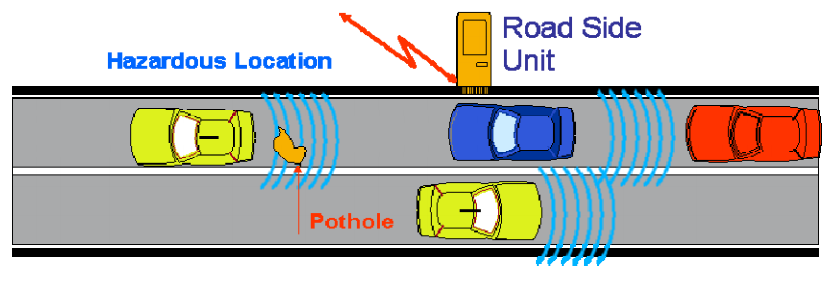
\includegraphics[width=0.95\textwidth]{content/images/06_use_cases/hln.png}
\caption{Hazardous Location C2C Notification Use Case \cite{etsi102638}}
\label{fig:hln}
\end{figure}

\subsection{Verkehrseffizienz}
Eins der Hauptziele von \acl{C2C} war die Steigerung der Verkehrseffizienz. Durch die bessere Leitung des Verkehrs entstehen weniger Staus auf den Straßen, was zu verminderten Stresssituationen für Fahrer führt. Es entstehen verkürzte Wartezeiten für die Teilnehmer am Verkehr und geringere Wartungskosten für die Straßen. Außerdem kann dadurch die Umwelt geschont werden und die Energiekosten gesenkt werden. 

\subsubsection{Enhanced Route Guidance and Navigation}
Navigation ist ein großes Thema das bereits über Navigationssysteme stark verbessert wurde. Enhanced Route Guidance and Navigation soll die Navigation noch einmal verbessern. Dies soll erreicht werden indem die Fahrdaten von den\ac{IRS} gesammelt und ausgewertet werden. Dadurch kann das Verkehrsaufkommen vorhergesagt werden. \ac{IVS}, deren potenzieller Weg an einer solchen Station vorbeiführt, können über die aktuelle Verkehrssitation informiert werden. Anhand dieser Informationen können sie den effektivsten Weg berechnen und Staus umfahren. Es ist auch möglich, dem Verkehr gezielt auf mehrere Straßen zu verteilen um die Verkehrsdichte auf den einzelnen Straßen zu reduzieren. Damit dieses Szenario funktioniert, müssen die \ac{IRS} die Möglichkeit besitzen, vorbeifahrende Fahrzeuge zu erkennen und zu informieren. 

\begin{figure}[htbp]
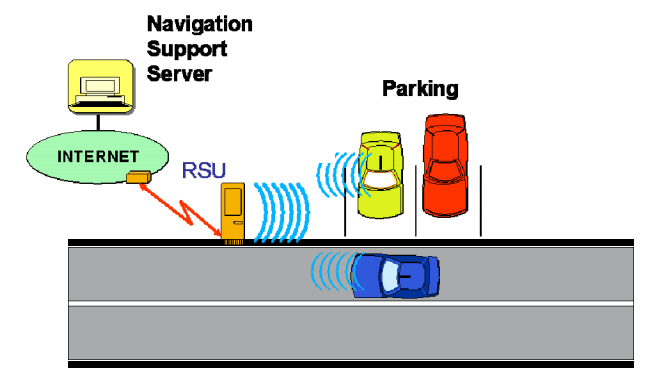
\includegraphics[width=0.95\textwidth]{content/images/06_use_cases/ergn.png}
\caption{Enhanced Route Guidance and Navigation Use Case \cite{etsi102638}}
\label{fig:ergn}
\end{figure}
\subsubsection{Green Light Optimal Speed Advisory}
Green Light Optimal Speed Advisory beschäftigt sich mit der optimalen Geschwindigkeit zwischen \acp{LZA}. Durch eine optimale Wahl der Geschwindigkeit von \ac{IVS} soll ermöglicht werden, dass die \ac{IVS} zwischen den \ac{LZA} mit einer konstanten Geschwindigkeit fahren. Ein permanentes Beschleunigen und Bremsen, sowie ein wiederholtes Anfahren soll vermieden werden. Um die Geschwindigkeit berechnen zu können, müssen die Schaltzeiten einer Kreuzung durch eine \ac{IRS} eingeholt werden können. Anhand der Schaltzeiten und den Abständen der \ac{IVS} kann die \ac{IRS} eine optimale Geschwindigkeit für die \ac{IVS} berechnen. Wenn alle \ac{IVS} die Geschwindigkeiten einhalten wird der Verkehrsfluss verbessert. Ein ruhiger Verkehrsfluss schont die Nerven der Fahrer und die Tankfüllungen der Fahrzeuge.

\begin{figure}[htbp]
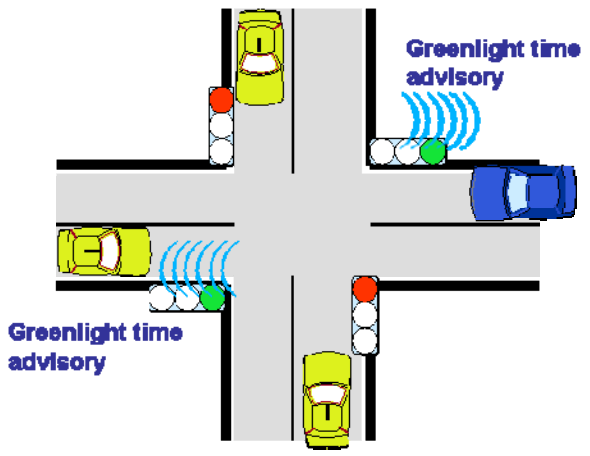
\includegraphics[width=0.95\textwidth]{content/images/06_use_cases/greenlight_opimalspeed.png}
\caption{Green Light Optimal Speed Advisory Use Case \cite{etsi102638}}
\label{fig:glos}
\end{figure}

\subsubsection{C2C Merging Assistance}
Beim Einfahren in den Verkehr kann es vorkommen, dass ein Fahrzeug den fließenden Verkehr stört. Dadurch entstehen nicht selten Rückstaus, die im schlimmsten Fall zu Auffahrunfällen führen. Eine Störung des Verkehrs soll über C2C Merging Assistance bereits beim Einfahren in den fließenden Verkehr verhindert werden. Sie wird verhindert, indem das Fahrzeug, das in den Verkehr einfließen möchte, die betroffenen Fahrzeuge darüber informiert. Die Fahrzeuge, die betroffen sind, sollen ihre Geschwindigkeit automatisch reduzieren. Zumindest sollen die Fahrer darüber informiert werden, wie sie sich am besten verhalten sollen. Dadurch kann der Verkehr weiter sauber fließen ohne dass es im Nachhinein zu einem Stillstand kommt. 

\begin{figure}[htbp]
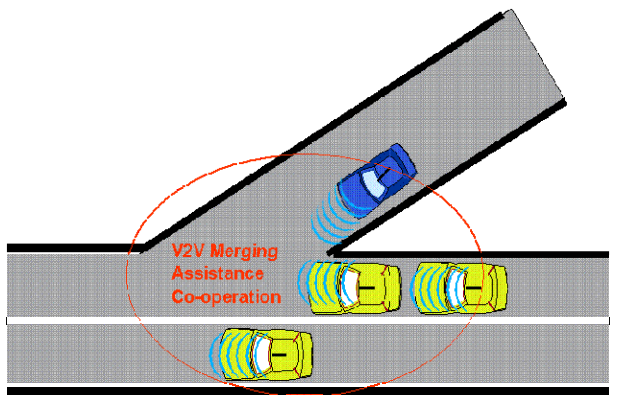
\includegraphics[width=0.95\textwidth]{content/images/06_use_cases/merging_assistance.png}
\caption{C2C Merging Assistance Use Case \cite{etsi102638}}
\label{fig:mergingassistance}
\end{figure}
\subsection{Infotainment und Andere}
Hier werden die Anwendungsfälle aufgeführt, die nicht zur Sicherheit oder Verkehrseffizienz beitragen, aber dennoch über die \ac{ITS} realisiert werden. Dazu gehören allgemeine Informationen, Entertainment oder Fahrzeugdaten, wie der Verbrauch reduziert werden kann. 

\subsubsection{Point of Interest Notification}
Dieser Anwendungsfall ist besonders für kommerzielle Werbezwecke interessant. Hier werden durch eine \ac{IRS} Informationen über, für den Fahrer interessante, Orte zu den umliegenden Fahrzeugen gesendet. Die Masse an Informationen kann situationsbedingt durch die \ac{IVS} gefiltert werden. Durch ein Reduzieren der Informationen auf die Relevanten kann der Fahrer entlastet werden. Tankstellen sind beispielsweise interessant, wenn der Kraftstoffstand der \ac{IVS} niedrig ist. Im Normalfall werden dem Fahrer keine Tankstellen angezeigt. Wenn der Kraftstoff aber niedrig ist, werden sie inklusive ihrer Öffnungszeiten und Preise angezeigt. Dadurch wird die Werbung deutlich effektiver, da die Zielgruppe richtig gewählt wird und sich in der unmittelbaren Umgebung aufhält.

\begin{figure}[htbp]
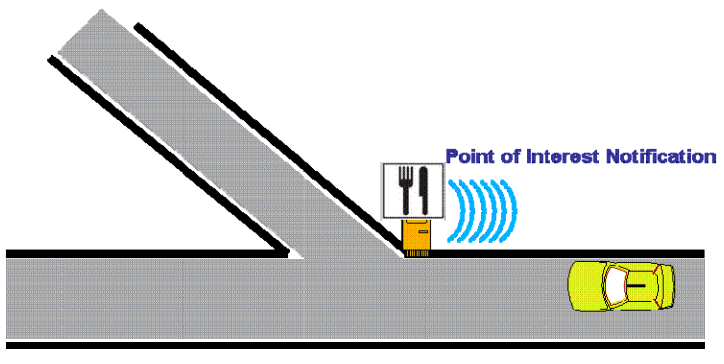
\includegraphics[width=0.95\textwidth]{content/images/06_use_cases/poin.png}
\caption{Point of Interest Notification Use Case \cite{etsi102638}}
\label{fig:poin}
\end{figure}

\subsubsection{Remote Diagnostics}
Der Remote Diagnostics Anwendungsfall beschreibt ein Szenario zum Warten der \ac{IVS}, ohne dafür in eine Werkstatt fahren zu müssen. Dadurch können vom Kundenservice Informationen über die \ac{IVS} abgerufen werden und mit Hilfe der Problembeschreibung des Fahrers kann schnell festgestellt werden, um welches Problem es sich handelt. Alle Daten über Werkstattbesuche und Probleme an der  \ac{IVS} sollen in einer Datenbank gespeichert werden. Durch diese Datenbank kann die Werkstatt, die die \ac{IVS} wartet, auslesen, was bereits an der \ac{IVS} gemacht wurde. Durch den Zugriff auf die Informationen können die Wartungszeiten, und damit auch die Wartezeiten in der Werkstatt, reduziert werden. Softwareupdates für \ac{IVS} müssen nicht mehr in Werkstätten durchgeführt werden, sondern können über \ac{ITS} geladen werden.

\begin{figure}[htbp]
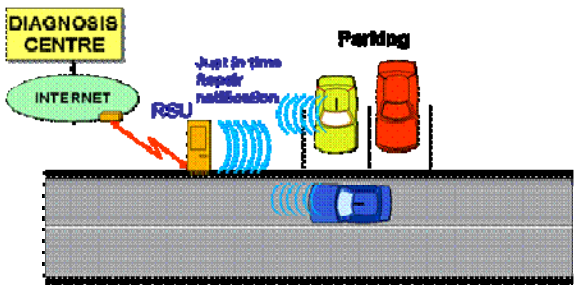
\includegraphics[width=0.95\textwidth]{content/images/06_use_cases/rds.png}
\caption{Remote Diagnostics \cite{etsi102638}}
\label{fig:redia}
\end{figure}
